\documentclass[12pt]{article}
\usepackage{fullpage,enumitem,amsmath,amssymb,graphicx,hyperref}
\usepackage[margin=1in]{geometry} 

\begin{document}

\begin{center}
{\Large CS221 Fall 2016 Project Progress: Scrabble AI}

\begin{tabular}{rl}
  Authors: & Colleen Josephson $\{$cajoseph$\}$ and Rebecca Greene $\{$greenest$\}$\\
\end{tabular}
\end{center}

\subsection*{Introduction}
Our project is to build a scrabble-playing AI, which is a popular
crossword board game in which players build words on a 15x15 board
using tiles representing letters. Since each player can make no direct
observations of the other player's rack, it is a \emph{stochastic
  partially observable game} [Russel and Norvig, 2003], which makes it
different from games like Othello, chess, or even Go, where players
has complete knowledge of the state of the game at any point. In
addition, the incredible number of possible moves renders typical
decision-tree models to be all but impossible. This makes Scrabble AIs
challenging to design. In this progress report we describe our model,
our preliminary algorithm, present preliminary experimental results,
and outline additional work we plan to do before the final
deadline. We consider the two-player case.


\subsection*{Model and Algorithms}
%% \subsection*{2.0 Overview of Scrabble}
%% Scrabble is a popular board game in which players build words on a 15x15 board using tiles representing letters. Different letters have different values, and the number of points a player recieves for forming a word is equal to the sum of the values of the tiles in the word, with multipliers depending on location on the board. There are a fixed set of tiles in the game, and at any point in the game, each player has access to at most 7 letter of these in their 'rack'.  When tiles are placed on the board they are replaced with ones drawn at random from a bag. If the players uses all 7 tiles this is called a 'bingo' and the move recieves a 50pt bonus, which can be about 1/8 of the total points in a tournament game.  Since each player can make no direct observations of the other player's rack, scrabble can be considerd a stochastic partially observable game [Russel and Norvig, 2003].  Thus it is very different from many games like othello, chess, or even go in which each player has complete knowledge of the state of the game at any point. In addition, the incredible number of possible moves renders typical decision-tree models to be all but impossible. \\
%% CAN ADD MORE TO THIS? 


For humans, one of the most important qualities to a good Scrabble
player is an extensive vocabulary. However, that is not by itself
sufficient for a competitive player. If a player optimizes for the
best score on every turn they tend to retain tiles that are more
difficult to use in play, leading to future racks that will produce a
lower score. The best Scrabble players try to maintain their rack in a
way that will be conducive to bingos\footnote{If the players uses all
  7 tiles this is called a 'bingo' and the move receives a 50pt bonus,
  which can be about 1/8 of the total points in a tournament game.} in
the future. Thus the general strategy for humans is to first look for
bingos, then look for potentially high-scoring positions, and to then
consider what remains on the rack.

For computers, which can be preprogrammed with the entire permissible
dictionary this is less of an issue. However, since that dictionary is
about 200,000 words long, searching through it for possible moves
becomes a nontrivial undertaking, and most scrabble AIs give
themselves a time limit to ensure reasonable progress of play.

Once a list of possible moves has been generated, the AI needs to select
the best move as a weighted decision of the score differential the
move would generate, the opportunities it would provide of the other
player, and the effect it would have on the future rack.

Scrabble AIs face the following challenges:

\begin{enumerate}
  \item \textbf{Move generation:} create a list of possible moves from
    the state of the board, the letters in the rack, and the allowable
    words in the dictionary. This is a nontrivial search problem.
    
  \item \textbf{Rack maintenance:} balance the tradeoff between getting
    the maximal score for a given turn with maintaining a rack that
    will be useful for future turns, which usually involves a weighted
    sum acquired with machine learning plus a number of Monte Carlo
    simulations.
    
  \item \textbf{Adversarial gameplay:} avoid creating opportunities
    for the other player to place high scoring words 
\end{enumerate}

Once the bag has been emptied (all tiles are either on the board or in
one of the racks), the game switches to being one with a completely
known state. At this point evaluation techniques like minimax become
useful to maximize score. This is commonly referred to as
\emph{endgame strategy}, and typically only state-of-the-art AIs go
into this level of detail.

\subsection*{Scrabble AI}
\subsubsection*{Move Generation}
To help solve the search problem, we're using an algorithm created in
the 1980s by Andrew Appel and Guy Jacobson, and remains the backbone
of most competitive scrabble AI players today. Appel and Jacobson
propose restructuring the Scrabble lexicon from a list of words into a
trie or prefix tree, where each node is a partial word, the children
of a node are words or partial words that can be created using that
node (see Fig. 1). All terminal leaves of the trie are words, as are
some interim nodes (e.g 'dog' vs. 'dogs'), and the value of a node is a
boolean indicating whether the sting is a full word in the dictionary.
%% We found the pytrie library rather helpful for implimenting this
%% algorithm, as it's CharTrie object was designed for implimentations
%% such as this, where the children of a node are held in a dictionary
%% that is indexed by letter (ex. startNode.children = {'c': <node
%%   object>, 'd': <node object>, 'e': <node object>). The maximim number
%%   of edges from a node is 26. Appel and Jacobson actually further
%%   reduce this to save on memory by combining nodes, but since we are
%%   now almost 30 years in the future, memory is less of a concern, so
%%   we decided to leave our dictionary as a trie.
  
To search for a move on a given board, the algorithm examines all
\emph{anchors}, where an anchor is the space to the left (or above) an
existing letter (for horizontal plays), or the space above an existing
letter (see Fig. 2). Since a move in Scrabble must attach to an
existing word (excepting the first move), only looking at possible
moves that extend from anchors greatly reduces the search space. After
each new move on the board, the AI should update it's list of anchor
squares.

Before a potential move is added to the list of generated moves, it
needs to be \emph{crosschecked} to ensure that new strings formed in
the orthogonal dimension also exist in the dictionary. For example, if
CAT and DOG are played horizontally right on top of each other, DC and
GT are not words so the move is not valid.  Since the crosscheck
results for a given tile remain static unless the tiles adjacent to it
change, the set of crosschecks needs only be updated once per move,
and only for the tiles immediately adjacent to new ones that have been
placed.

The heart of the algorithm is a backtracking search with constraints
that the final result must be a valid word (enforced by the structure
of the trie itself), all crosschecks pass, and the new letters placed
on the board come from the player's rack. The search algorithm has two
recursive parts: ExtendLeft and ExtendRight. Below is pseudocode for
the backtracking algorithm to place a horizontal word:\\

\quad ExtendRight (PartialWord, node N, square):

\quad\quad if square is not empty:

\quad\quad\quad if the letter l in square is an edge of N (PartialWord + l is a node):

\quad\quad\quad\quad ExtendRight(PartialWord + l, N.children[l], nextSquare)

\quad\quad else:

\quad\quad\quad if PartialWord is a word: LegalMoves.append(PartialWord)

\quad\quad\quad for each letter l that is in rack, s an edge out of N,in the cross-check set of square:

\quad\quad\quad\quad\quad remove l from the rack

\quad\quad\quad\quad\quad ExtendRight(PartialWord + l, N.children[l], nextSquare)

\quad\quad\quad\quad\quad put tile l back into the rack\\

Thus all possible words from the right of an anchor tile are produced. For out example in Figure 2, this would be 


The next part of the algorithm is ExtendLeft, places tiles to the left
of the anchor point and then calls ExtendRight to see what words can
be formed using those placements. 'Limit' is the number of blank tiles
between the current anchor point and the preceeding anchorpoint (or the end of the board), capped at the rack size of 7. The ExtendLeft pseudocode: \\

\quad ExtendLeft(PartialWord, node N, square, limit):

\quad\quad ExtendRight(PartialWord, N, square)

\quad\quad if limit $>$ 0: 

\quad\quad\quad for each letter l in rack that is an edge of N: 

\quad\quad\quad\quad remove l from the rack

\quad\quad\quad\quad ExtendLeft(l+PartialWord, N' =
N.children[l], nextSquare, limit -1)

\quad\quad\quad\quad put tile l back into the rack\\
			
To generate a list of all legal moves for a given board, call
LeftExtend("", root node, anchorSquare, Limit) on all anchors.

%Based off appel-jacobsen is move generation algo, we will do a
%backtracking search on a trie where the letters are edges and nodes
%are partial words/words (leaf nodes are words). The maxmum number of
%edges from a node is 26. The trie is pre-computed from the dictionary.

%The trie itself enforces the constraint of each tile-placement being
%the substring of a word in the dictionary. The backtracking search
%will enforce the other constraints, namely:
%-selected letters must come from the player's tile set
%-word must not form a non-word with another part of the board
%-word must fit on the board

%From there, we will generate all possible moves (or some randomized
%subset of them, if this is far too time-consuming) and choose maximal
%weight move, where the weight is the standard Scrabble score
%function. Some Scrabble AIs have additional heuristics in the score,
%such as weighting words based on how they impact the tile rack. We
%stuck with the simple scording function for the first pass, but may
%conisder additional heuristics for the final result.

\subsubsection*{Rack Maintenance and Adversarial Gameplay}
The next step of the problem is to try to decide which of the legal
moves to make, given consideration of score, maintaining a reasonable
rack, and not giving any advantages to the opponent. This is done
through a combination of Monte Carlo simulation and linear predictors
with learned weights. The raw score of a move is as a function of tile
values and multipliers on the board, plus any resulting multi-word
bonuses or bingos. However, the point differential (TODO: DEFINE THIS)
as a result of the move (which is far more important) is best computed
through simulation. For each of the top raw-scoring moves, the AI runs
a number of Monte Carlo simulations playing against itself with
probable opponent racks. Since the turnover rate of racks is so high,
and the computation required per move is rather extensive, most
competitive AIs run their models with a search depth $\geq 3$. Our
preliminary algorithm does not implement this, but we would like to
add it for the final product.

Many Scrabble AIs don't try to make any assumptions about the opposing
player's rack, and just assign the opponent random unseen letters when
running simulations. However, it is possible to use Bayes' algorithm
to make a probabilistic model of the tiles a player had on their rack
at the start of a turn given the move they made during that turn.%% This
%% is equivalent to having a model of many of the tiles the opposing
%% player will have on their rack for the next turn (the rest are
%% filled in at random from the letter bag).
For instance, if the opposing player used the letters 'C, T' to attach
to an A and make "CAT", it is unlikely that they left an S on their
rack, because otherwise they would have played "C,T,S" to make "CATS",
which is a higher scoring word. More formally $P(leave | play) =
\frac{P(play | leave)P(leave)}{P(play)}$, where P(leave) is the
probability that certain tiles were left on the rack. When an AI's
Monte Carlo simulations draw from this probability space rather a
random assignment, the algorithm has better performance on a level
that is statistically significant(TODO:cite paper).

	
%% Now that the scores have been computed by simulation, they are weighed
%% along with heuristics for rack maintaince to select the best move to
%% use. The features extracted for this purpose are:

%% \begin{enumerate}
%%   \item counts of tile(A), duplicated tile (BB), and triples of a
%%     tile(CCC) for different letters.  It is apparent that 'UU' would
%%     be less desirable than 'AA', for example
%%   \item balance of vowels and constants (which has been proven to be
%%     an important factor in weight maintince
%%   \item 'QU' combination (???)
%% \end{enumerate}

%% The weights for these features are learned by initially setting them all to zero, and having the AI play itself, running stochastic gradient descent using the difference in score at the end of the game. 

For a concrete example of the backtracking search constraints, please
see the next section.

\subsubsection*{Examples and Preliminary Data}
For our initial attempt at the Scrabble AI, we successfully
implemented the Appel/Jacobson algorithm, but didn't consider any
features besides the raw score when selecting a move, and didn't
attempt to do any opponent modeling.  To evaluate our AI's
performance, we had it play an open-source scrabble AI 'Quackle',
which has beaten human champions. Because the Quackle code is in C++,
it is possible to make our AI play the Quackle AI in an automated
manner, and indeed necessary to get a large dataset for our final
paper. Unfortunately, because of time constraints, the interface
between the two AIs hasn't been built yet, so we have a collection of
results obtained by manually interfacing the two AIs, the results are
presented below in Table 1.  We will have automated AI vs AI
capability to create a larger dataset for the final result. \\

\begin{table}[h]
  \centering
\begin{tabular}{c|l|l|l|l|l|l|l|l}
  \textbf{CS221 AI} & 234 & 249 & 236 & 181 & 235 & 321 & 279 & \textbf{Average Score: } 247.7 \\\hline
  \textbf{Quackle}  & 396 & 278 & 264 & 303 & 386 & 441 & 417 & \textbf{Average Score: } 355\\
\end{tabular}
\caption{Raw scores and averages for 7 CS221 vs. Quackle games}
\end{table}

Here is an example of the input and output of our AI. On the left is an input board where the Quackle AI has played COMPOTE. Underneath is our AI's rack. On the right is the move our AI chose to mak, RAJES. Beneath the figures is an example of the LegalMoves list, over which the AI maximizes. 

\begin{figure}[h]
  \minipage{0.5\textwidth}
    \centering
  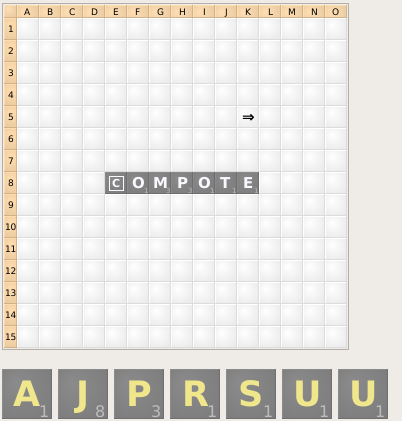
\includegraphics[scale=0.5]{exampleboard}
  \caption{Example of an input board}
  \endminipage
  \minipage{0.5\textwidth}
      \centering
  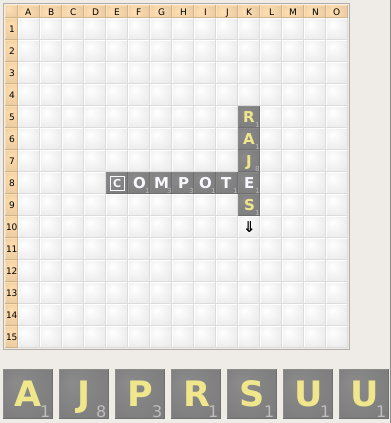
\includegraphics[scale=0.5]{exampleplay}\\
   \caption{Our AI plays 'RAJES' on the board}
  \endminipage{}
\end{figure}

The output of
\texttt{There are 191 legal moves: [('JO', (6, 8), 'v', 17), ...,  ('RAJES', (4, 10), 'v', 36), ('TRAPS', (7, 9), 'v', 9)])\\
max word RAJES with score 36}



\subsubsection*{Future Work}
One of our first tasks moving foward will be to find a way to
interface our AI with Quackle so that they can play each other, and we
can more easily see the results of our algorithm. We will also be able
to use scores against Quackle as a metric for using stochastic
gradient descent to create weight vectors for our rack-maintaince
heuristics. After that, our goal is to have the AI use depth-2 monte
carlo simulations to determent the point differential created by a
word, instead of using the raw score of the tiles. If we have time
we'll create a probalistic model for the opposing player to make the
monte carlo simulations more accurate.
\section*{Appendix}
\begin{center}
  From Appel-Jacobsen '86\\
  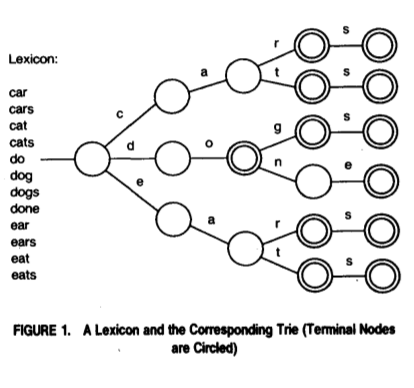
\includegraphics[scale=0.6]{trie}\\
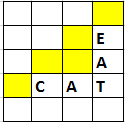
\includegraphics{anchorexample}\\
Figure 3: An Example of Anchor Squares
\end{center}
\end{document}
